\documentclass{article}
\usepackage[utf8]{inputenc}
\usepackage{amsthm}
\usepackage{amsmath}
\usepackage{verbatim}
\DeclareMathOperator*{\argminA}{arg\,min}
\title{From MLE of Gaussian to linear regression}

\date{}
\usepackage{natbib}
\usepackage{graphicx}
\usepackage{amsthm}
\usepackage{amssymb}
%\newtheorem{theorem}{Theorem}
\newtheorem{theorem}{Theorem}[section]
\newtheorem{corollary}{Corollary}[theorem]
\newtheorem{lemma}[theorem]{Lemma}
\graphicspath{ {/} }
\theoremstyle{remark}
\newtheorem*{remark}{Remark}

\theoremstyle{definition}
\newtheorem{definition}{Definition}[section]
\newtheorem{example}{Example}[section]



\usepackage[utf8]{inputenc}
\usepackage[english]{babel}

\usepackage{blindtext}



\usepackage{amsthm}

\begin{document}
	
	\maketitle
	
	\section{MLE of Gaussian}
	Say we have physical heights of students and we want to fit Gaussian distribution to it. E.g. we have observations $X = \{x_1, x_2,...x_n\} =  \{ 165 \text{ cm}, 193 \text{ cm},...177 \text{ cm}\}$.
	
	Our distribution is $N(\mu, \sigma^2)$ with PDF 
	$$
	f(x) = \frac{1}{\sqrt{2 \pi \sigma^2}} \exp \left( \frac{\left( x-\mu \right)^2 }{2\sigma^2} \right)
	$$
	
	We may emphasize that the part $\frac{1}{\sqrt{2 \pi \sigma^2}}$ does not depend on $x$, and that the charasteristic shape of Gaussin is given (ommiting parameters) by the function $\exp(-x^2)$ (easy to remember, compared to the whole formula for PDF. This is also part from which the sum of squares will appear, after $\exp(.)$ cancels with $\log(.)$ in negative log-likelihood).
	
	We recall the definition of likelihood function, 
	$$L(\mu, \sigma^2) = \prod_{i=1}^{n} f(x_i | \mu, \sigma^2)$$ 
	We may emphasize that the product comes from multiplication of probability densities of independent events, and that the observations are assumed to be i.i.d. (identically independently distributed). We may plot the likelihood e.g. as function of $\mu$ (for some given numerical values of $X$ and $\sigma^2$).
	
	We recall that for functions taking positive values,
	 $$\arg \max f(x) = \arg \max \log(f(x))$$
	 so if we want to maximize likelihood, we may equivalently maximize log-likelihood
	 $$
	 l(\mu, \sigma^2) = \log \left( L(\mu, \sigma^2) \right) = \log \left( \prod_{i=1}^{n} f(x_i | \mu, \sigma^2) \right) = \frac{n}{\sqrt{2 \pi \sigma^2}} + \frac{1}{2\sigma^2} \sum_{i=1}^{n} (x-\mu)^2
	 $$
	 So here we see the sum of squares term $\sum_{i=1}^{n} (x-\mu)^2$, plus bunch of stuff that do not depend on $\mu$.
	 
	 We may maximize $l(\mu, \sigma^2)$ with respect to $\mu$ by taking derivative and setting it to $0$, result is the empirical mean $\hat{\mu} = \frac{1}{n}\sum_{i=1}^{n} x_i$.
	 
	 We may plot also the log-likelihood, show that its arg max is the same as of likelihood, and how are these two functions related.
	 
	 \section{(Optional) intermediate step: 2 separate Gaussians}
	 Now we may say: wait a minute, one Gaussian for whole population is maybe not a good model. E.g. men are taller than woman on average, so we may fit one distribution for men and another for woman. And if we know the sex of person, we can use it as explanatory variable, i.e. to choose the corresponding Gaussian to make prediction about person's height.
	 
	 This can be seen as having two means, $\mu_1$ and $\mu_2$. Equivalently, parametrize $\mu = \beta_0 + \beta_1 \times \text{is\_men}$, where $\text{is\_men}$ is  abinary variable with value $1$ for men and $0$ otherwise.
	 
	 Visualize these two Gaussian + data like this, to prepare for the 'full' linear regression setup.
	\\
	{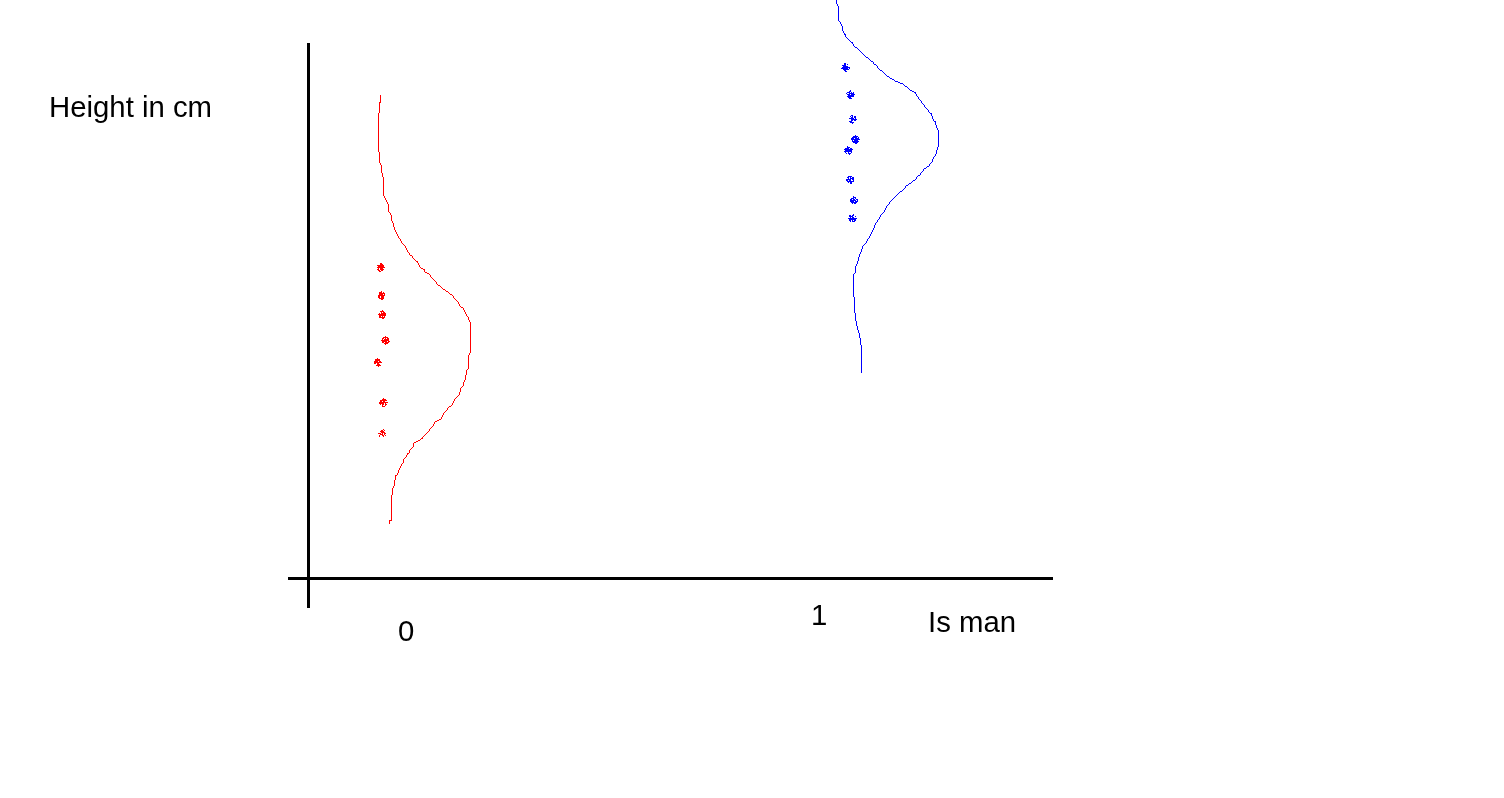
\includegraphics[width=15cm]{two_gaussians.png}
	\\
	
	\section{Generalize to full linear regression model}
	Discuss that instead of having one model for men and one for woman, we may also account for continuous explanatory variable , e.g. account for age in years as $\mu = \beta_0 + \beta_1 \times \text{age}$. Or, more generally, $\mu = \mathbf{\beta}^\mathsf{T} \mathbf{x}$ where $\mathbf{x}$ is arbitrary vector of explanatory variables.
	
	Visualize the loss function of multi-variable linear regression (2 explanatory variables + functional value, i.e. 3-d plot), recall that it have analytical solution but we may also minimize numerically. Recall that it's same concept as in part 1 and that the sum of square error still comes from Gaussian.
	
\end{document}
